\documentclass[margin=0.1in]{standalone}
\usepackage{tikz}
\usepackage{amsfonts}
\usepackage{amsmath}
\usepackage{amssymb}
\begin{document}

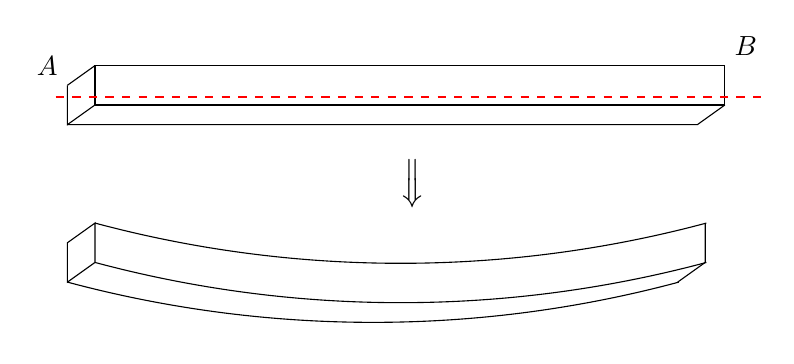
\begin{tikzpicture}[>=latex]
% PRIMER VIGA
	\draw (0,0) rectangle (8,0.5) node [above right] {\(B\)};
	\coordinate (P) at (-0.35,0.25);
	\draw (P) node [above left] {\(A\)} --++ (0,-0.5) -- (0,0);
	\draw (P) -- (0,0.5);
	\draw (P) ++ (0,-0.5) --++ (8,0) -- (8,0);
	\draw [thick , red, dashed] (-0.5,0.1) --++ (9,0);
	\node [rotate = -90] at (4,-1) {\large \(\;\implies\;\)};
% SEGUNDA VGA
	\begin{scope}[shift={(0,-2)}]
		\draw (-0.35,0.25) --++ (0,-0.5) -- (0,0) -- (0,0.5) -- cycle;
		\draw (0,0) arc (255:285: 15 cm);
		\draw (0,0.5) arc (255:285: 15 cm);
		\draw (-0.35,-0.25) arc (255:285: 15 cm);
		\draw [xshift=7.75cm] (-0.35,-0.25) -- (0,0) -- (0,0.5);
	\end{scope}
\end{tikzpicture}

\end{document}
